
\documentclass[template=tabling,81pt,headonall]{azmoon}
\usepackage{xepersian}
\usepackage{amsfonts}
\usepackage{graphicx}
\graphicspath{ {./images/} }
\settextfont{Yas}
\setdigitfont{A Iranian Sans}
\usepackage{fontawesome5}

\printanswers
    \teacher{محمد صالح علی اکبری}
    \teachertitle{دبیر}
    \city{گناباد}
    \schooltitle{متوسطه دوره دوم}
    \school{شاهد امام (ره)}
    \grade{دهم}
    \branch{-}
    \topic{ریاضی}
    \examdate{10/07/1402}
    \answertime{25 دقیقه}
    \begin{document}
	\begin{questions}
		\nointerlineskip%
		\vskip-\baselineskip
		\question{%
 نقطه A به فاصله ۴ واحد از خط d قرار دارد. نقاط M و M' روی خط d و به فاصلة ۵ از نقطه A قرار دارند. فاصله MM' کدام است؟
    \begin{fourchoice}[4]\choice{6}
\choice{3}
\choice{5}
\choice{4}
\end{fourchoice}
    }
\question{%
دو نقطه A و B به فاصله ۴ از هم قرار دارند. فقط یک نقطه در صفحه وجود دارد که به فاصله ۳ از A و  $و2a-1$ از B قرار دارد. مقدار a کدام است؟
    \begin{fourchoice}[4]\choice{1}
\choice{2}
\choice{3}
\choice{1 یا 4}
\end{fourchoice}
    }
\question{%
 نقاط A و B به فاصله ۱۳ از هم قرار دارند. نقاطی که به فاصله ۱۲ از A و به فاصله ۵ از B می‌باشند را معلوم کرده و از آن‌ها به A و B وصل می‌کنیم. مجموع مساحت‌های شکل‌های حاصل کدام است؟
    \begin{fourchoice}[4]\choice{30}
\choice{120}
\choice{60}
\choice{90}
\end{fourchoice}
    }
\question{%
مرکز همه دایره‌هایی که از دو رأس A و B از مربع ABCD می‌گذرند. چگونه‌اند؟ (سؤال دو گزینه درست دارد)
    \begin{fourchoice}[2]\choice{روی دایره‌ای به قطر ضلع AB قرار دارند.}
\choice{روی خطی موازی ضلع AB قرار دارند.}
\choice{روی عمودمنصف ضلع CD قرار دارند.}
\choice{روی خطی عمود بر ضلع AB قرار دارند.}
\end{fourchoice}
    }
\question{%
مربع ABCD به ضلع ۴ مفروض است. مرکز دو دایره از مجموعه دوایری به شعاع ۵ که همگی از رأس A می‌گذرند روی محیط مربع قرار دارد. فاصله مرکزهای این دو دایره کدام است؟
    \begin{fourchoice}[4]\choice{2}
\choice{2}
\choice{$\sqrt{3}$}
\choice{$\sqrt{2}$}
\end{fourchoice}
    }
\question{%
در شکل مقابل، چهارضلعی ABCD مستطیل است و نقاط M ، N و P که روی اضلاع مستطیل و امتداد آن‌ها هستند به فاصله برابر از رأس A قرار دارند. اگر $BM=7$، $MC=8$ و $DP=10$ باشند. طول پاره‌خط NC کدام است؟ \\ 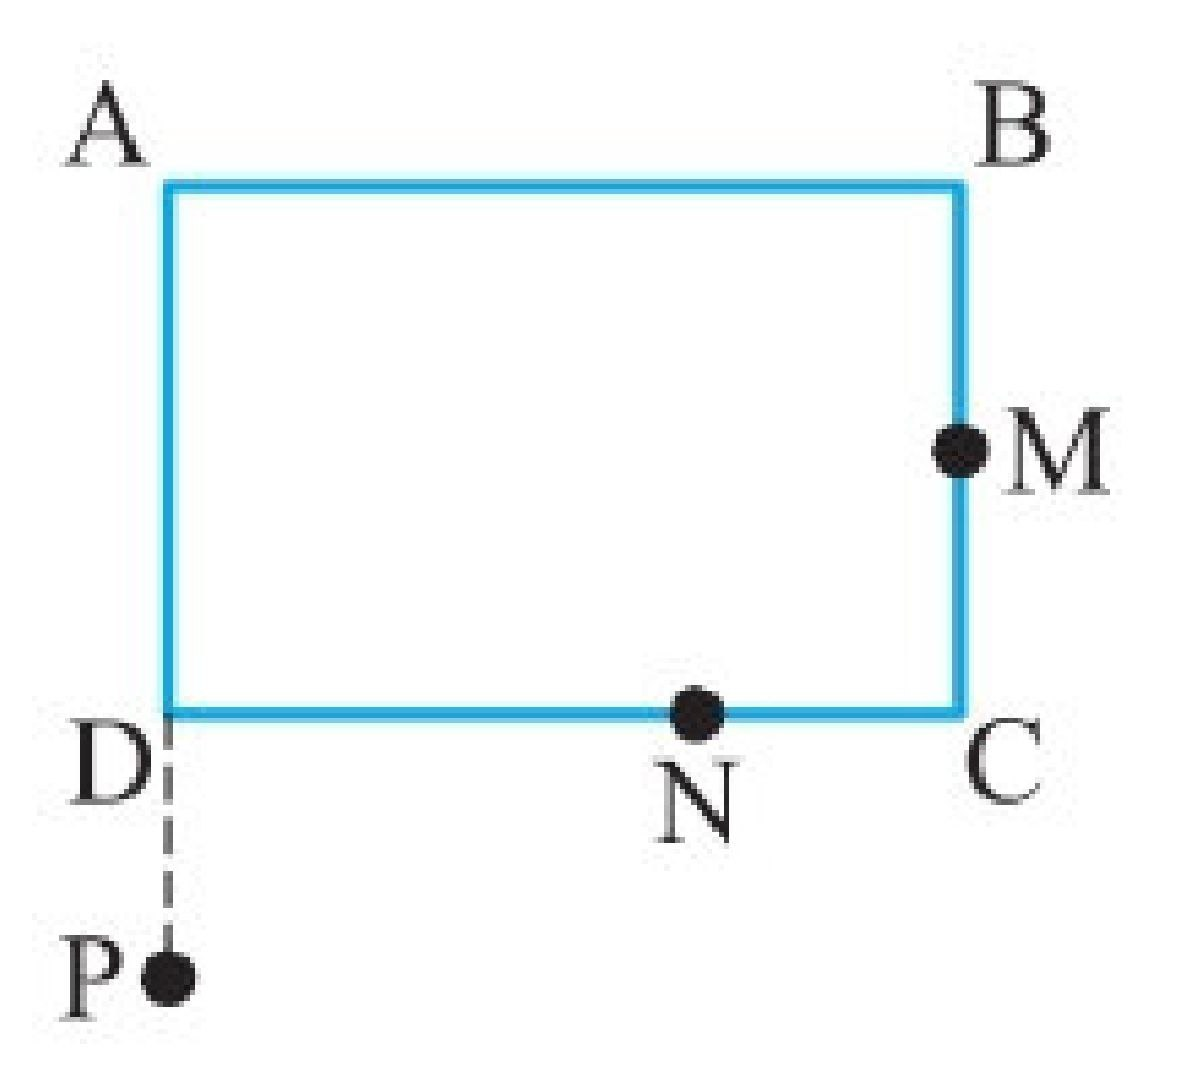
\includegraphics[scale = 0.08]{photo_2023-10-02_00-39-47}
    \begin{fourchoice}[4]\choice{4}
\choice{3.5}
\choice{3}
\choice{2}
\end{fourchoice}
    }
\question{%
روی محیط مستطیلی به ابعاد ۴ و 8، دو نقطه وجود دارد که به فاصله ۵ از یک رأس آن قرار دارند. فاصله این دو نقطه از هم کدام است؟
    \begin{fourchoice}[4]\choice{$2 \sqrt{7}$}
\choice{$3\sqrt{2}$}
\choice{4}
\choice{$2\sqrt{5}$}
\end{fourchoice}
    }
\question{%
نقطه M درون مربع ABCD به ضلع ۴ قرار دارد. اگر نقاط A، B و وسط ضلع CD از نقطه M به یک فاصله باشند. فاصله M تا مرکز مربع کدام است؟
    \begin{fourchoice}[4]\choice{$0.5$}
\choice{1}
\choice{$1.5$}
\choice{$2.5$}
\end{fourchoice}
    }
\question{%
خط d بر دایره C مماس است. m نقطه روی دایره وجود دارد که از خط d به فاصله معلوم L هستند. m کدام نمی‌تواند باشد؟
    \begin{fourchoice}[4]\choice{صفر}
\choice{1}
\choice{2}
\choice{3}
\end{fourchoice}
    }
\question{%
در شکل مقابل AD نیمساز زاویه A است. اگر $BD=4$ و$S_{ABD} +12 = S_{ADC}$ باشند، طول پاره‌خط CD کدام است؟ \\ 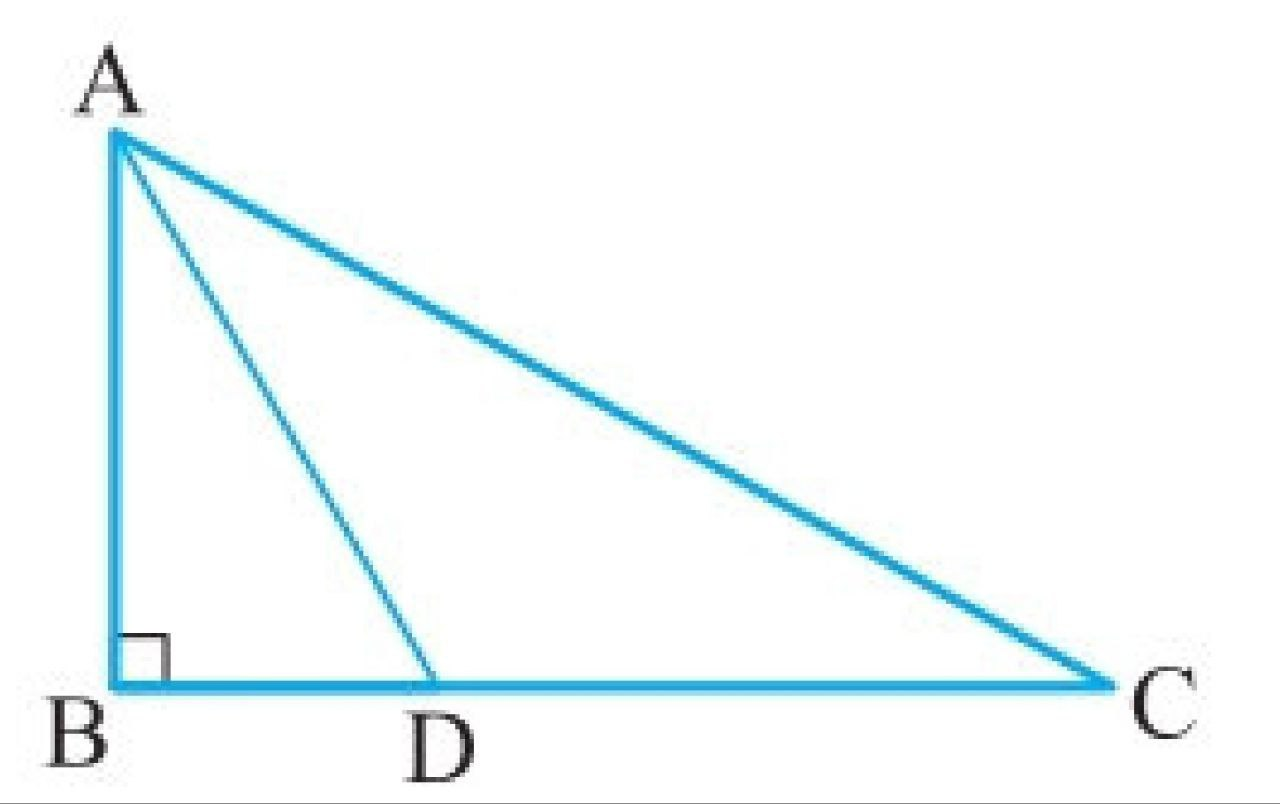
\includegraphics[scale = 0.08]{photo_2023-10-02_00-39-16}
    \begin{fourchoice}[4]\choice{7}
\choice{$5\sqrt{2}$}
\choice{$2\sqrt{13}$}
\choice{8}
\end{fourchoice}
    }
\end{questions}
    \end{document}
    